\documentclass[11pt,a4paper]{article}

\usepackage{graphicx}
\usepackage{url}
\usepackage{listings}
\title{Generate PWM for velocity control of a Servo Motor}
\author{e-Yantra Team}
\date{\today}

\begin{document}
	\maketitle
	\newpage
	\tableofcontents
	\newpage
	
	\section{Objective}
	In this tutorial we shall learn to control the angle of rotation of a servo motor(using PWM) interfaced with Raspberry Pi. 
	
	\section{Prerequisites}
	\begin{itemize}
		\item Python programming skills
    \end{itemize}
	
	\section{Hardware Requirement}
	\begin{enumerate}
		\item Raspberry Pi (I will be using Version 2 Model B)
		\item MCP23017
		\item Power adapter
		\item Servo motor (I will be using the Futuba make)
		\item Connecting wires
		\item Bread board
	\end{enumerate}
	
	\section{Software Requirement}
	\begin{enumerate}
		\item PyScripter (version 2.7 or above)
		\item Mobaxterm (for windows user)
	\end{enumerate}
	
	\newpage
	\section{Theory and Description}
	Servo motor is normally a simple DC motor which is controlled for specific angular rotation with help of additional servomechanism (a typical closed loop feedback control system). 
	\newline
	In short Servo motor is a special type of motor which is automatically operated up to certain limit for a given command with help of error-sensing feedback to correct the performance.[1]
	
	\begin{figure}[h!]
		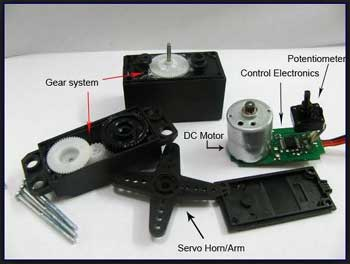
\includegraphics[scale=0.8]{sm.jpg}
		\centering
		\caption{[1]}
	\end{figure}
	 
	\newpage
	\flushleft
	\textbf{Angle of Rotation}
	
	The angle (of mechanical rotation) is determined by the width of an electrical pulse that is applied to the control wire. This is a form of pulse-width modulation, however servo position is not defined by the PWM duty cycle (i.e., ON vs OFF time) but only by the width of the pulse. The servo expects to see a pulse every 20 ms, however this can vary within a wide range that differs from servo to servo. The width of the pulse will determine how far the motor turns. For example, a 1.5 ms pulse will make the motor turn to the 90 degree position (neutral position). [2]
	

	
	The minimal width and the maximum width of pulse that will command the servo to turn to a valid position are functions of each servo. Different brands, and even different servos of the same brand, will have different maximum and minimums. Generally the minimum pulse will be about 1 ms wide and the maximum pulse will be 2 ms wide.[3]
	
	\begin{figure}[h!]
		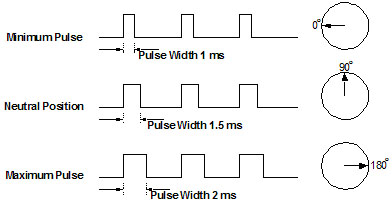
\includegraphics[scale=0.7]{anr.jpg}
		\centering
		\caption{[3]}
	\end{figure}
	
	 Another parameter that varies from servo to servo is the turn rate. This is the time it takes from the servo to change from one position to another. The worst case turning time is when the servo is holding at the minimum rotation and it is commanded to go to maximum rotation. This can take several seconds on very high torque servos.[3]
	 
	 \newpage
	 \textbf{Pin Diagram}
	 \begin{figure}[h!]
	 	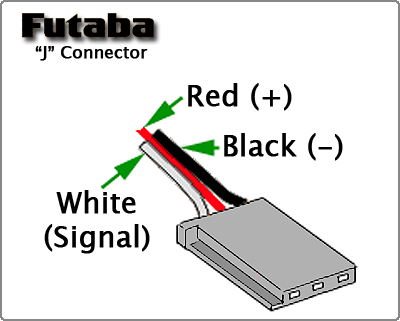
\includegraphics[scale=0.7]{fc.png}
	 	\centering
	 	\caption{[3]}
	 \end{figure}
	 
	\newpage
	\section{Experiment}
	
	\textbf{PWM generation for controlling the angle of rotation of a Servo motor interfaced with R-Pi}
	
	In this experiment we will be programming a servo motor using software pwm generation technique.
	
	\begin{figure}[h!]
		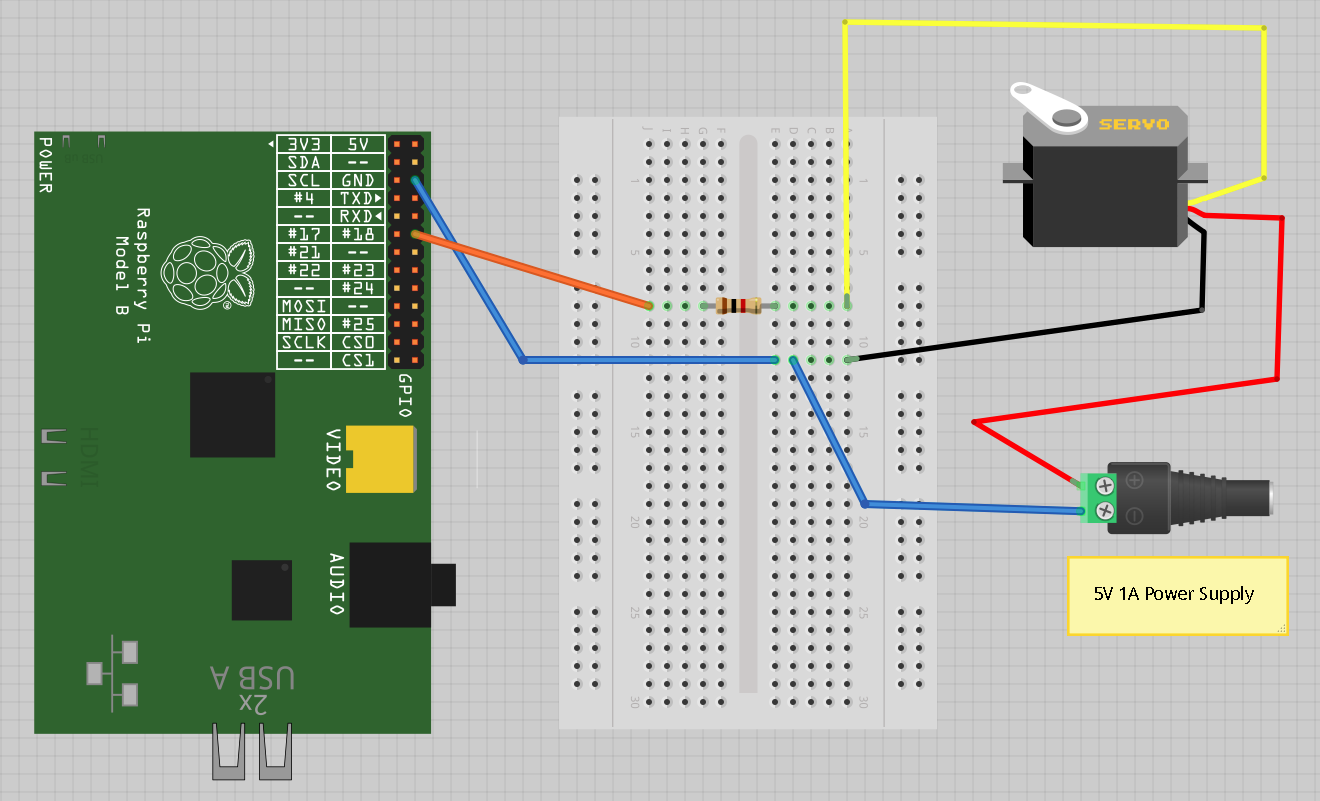
\includegraphics[scale=0.8]{i.png}
		\centering
		\caption{[4]}
	\end{figure}
	
	In this figure the enable pin of the motor is connected to GPIO 11 of R-Pi.
	
	\vspace{0.3cm}
	\textbf{Code}
	\vspace{0.3cm}
	
	\lstinputlisting[language=Python]{servo.py}
	
	\newpage
	\section{Appendix}
	
	\subsection{Raspberry Pi 2 Pin-out Diagram}
	\begin{figure}[h!]
		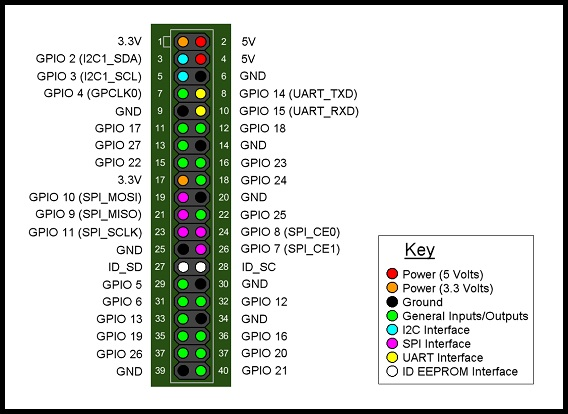
\includegraphics[scale=0.6]{RaspberryPi2_pinout.jpg}
		\centering
		\caption{[4]}
	\end{figure}
	
	\subsection{MCP23017 datasheet}
	
	\url{http://ww1.microchip.com/downloads/en/DeviceDoc/21952b.pdf}
	
	\subsection{PWM}
	In order to learn more about PWM kindly refer \url{https://github.com/eyantrainternship/eYSIP_2015_RaspberryPi-Development-Board/tree/master/Task%206}
		
    \newpage 
	\section{References}
		\begin{enumerate}
			\item \url{http://www.electrical4u.com/servo-motor-servo-mechanism-theory-and-working-principle/}
			\item \url{https://en.wikipedia.org/wiki/Servo_control}
			\item \url{https://www.servocity.com/html/how_do_servos_work_.html#.VZsqx_mqqkp}
			\item \url{http://razzpisampler.oreilly.com/images/rpck_1001.png}
			\item  \url{http://data.designspark.info/uploads/images/53bc258dc6c0425cb44870b50ab30621}
		\end{enumerate}
	
\end{document}



